\section{Introduction}

As we can see before, the sediment mass conservation equation, i.e. Exner equation \eqref{eq:exner}, only describes the time-evolution of $Z_b$ which is the bottom elevation (the lowest point of the river cross-section). More precisely, the numerical scheme \eqref{eq:exner-scheme} computes
\begin{equation}\label{eq:exner-sediment-volume}
\Delta V_i^{n+1} \equiv V_i^{n+1} - V_i^n
\end{equation}
the eroded/deposited volume of sediments at cell $i$ during the time $t^n$ to time $t^{n+1}$. As a consequent, an additional closure is needed in order to describe the evolution of river cross-section.

Several closures can be found in the literature. The simplest closure may be a {\em flat} deposition and an {\em uniform} erosion; the height of erosion at each point on the river cross-section can even be weighted in according with the efficient shear stress $\tau_{eff}$. An another one consists in applying an uniform evolution for both deposition and erosion cases.

Once the geometry of cross-sections are modified by erosion or deposition, the {\em planimetrage functions} -- vertical discretization of cross-sections -- need to be re-calculated at each time step
\begin{itemize}
\item $B(z)$: width of cross-section,
\item $S(z)$: area of cross-section,
\item $P(z)$: perimeter of cross-section,
\end{itemize}
corresponding to a given elevation $z$. As remarked before, this becomes costly for long-term simulations with a lot of bed evolutions (which can represent up to more than 90\% of the total calculation time of \courlis).

In the following, we are interested by the simple closures allowing direct analytic computation of planimetrage functions $B^{n+1}, S^{n+1}, P^{n+1}$ at time $t^{n+1}$ from time $t^n$ (available  functions $B^n, S^n, P^n$), or from the initial time $t^0$ (functions $B^0, S^0, P^0$ are given by \mascaret after initialization step).  The choice of these closures is given with the keyword \telkey{OPTION D'EVOLUTION DE PROFIL} or \telkey{OPTION FOR PROFILE EVOLUTION}.

\section{Option 1: uniform erosion -- flat deposition}

\subsection{Keywords}
\begin{itemize}
\item \telkey{OPTION FOR PROFILE EVOLUTION = 1} (default)
\end{itemize}

\subsection{Profile evolution}
Evolution of the river bottom is not applied in the same way for erosion and for deposition :
\begin{itemize}
 \item Evolution due to erosion is applied uniformely on all points of the river bottom located under the free surface ;
 \item Evolution due to deposition is applied horizontally (at constant elevation). For each horizontal deposition surface, the corresponding elevation is computed by linear interpolation of the curves generated by vertical discretization (cf Section \ref{planim}).
\end{itemize}

\begin{figure}[htb!]
    \centering
    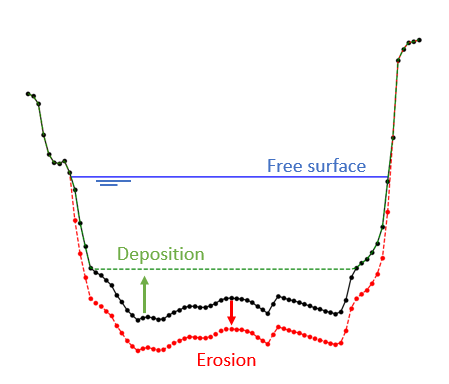
\includegraphics[width=0.45\textwidth]{./graphics/erosion_deposition.png}
    \caption{Flat deposition and uniform erosion}
    \label{fig:depo_ero2}
\end{figure}

\subsection{Planimetrage functions}
wip

\section{Option 2: uniform erosion -- uniform deposition}

\subsection{Keywords}
\begin{itemize}
\item \telkey{OPTION FOR PROFILE EVOLUTION} = 2
\item \telkey{FILE FOR THE WIDTH OF EROSION} = largeur.xlim
\end{itemize}

\subsection{Profile evolution}
For a cross-section $i$, a value $B_i$ {\em width of erosion} or the positions $x_i^L, x_i^R$ on the left and the right river banks have to be prescribed in the \telkey{FILE FOR THE WIDTH OF EROSION}. The format of this later file is closely derived from that of geoCourlis as follows:

\begin{figure}[htb!]
\begin{verbatim}
Profil Bief_1 Profil_1 X1     Profil Bief_1 Profil_1 X1 [B1 or X1L X1R]
Profil Bief_1 Profil_2 X2     Profil Bief_1 Profil_2 X2 [B2 or X2L X2R]
...                           ...
\end{verbatim}
\caption{geoCourlis file (left) and (right) format of \telkey{FILE FOR THE WIDTH OF EROSION}.}
\end{figure}

The mechanism for erosion and deposition cases are illustrated on Fig. \ref{fig:option-uni-depo-ero}. The current geometry is derived from initial cross-section. In the case of erosion, the part of initial cross-section lying between $x^L$ and $x^R$ is uniformly displaced downward with a thickness $\delta z_i$. For the opposed case, this part of initial cross-section is uniformly moved upward by $\delta z_i$ and completed by horizontal jonctions at $x^L$ and $x^R$.

\begin{figure}[htb!]
    \centering
    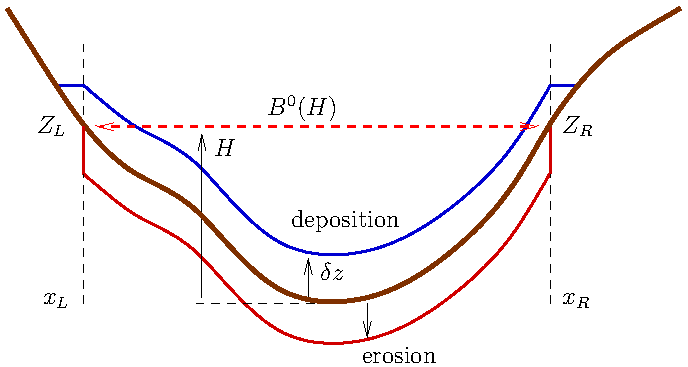
\includegraphics[width=0.5\textwidth]{./graphics/option-uni-depot-ero.pdf}
    \caption{Uniform deposition and uniform erosion, with the brown curve corresponding to the initial profile}
    \label{fig:option-uni-depo-ero}
\end{figure}

\subsection{Planimetrage functions}
The planimetrage functions $B^{n+1}, S^{n+1}, P^{n+1}$ can be directly computed from those of initial time $B^0, S^0, P^0$.

First, we compute from $B^0$ the height $H_i$ associated to the given width of erosion $B_i$ by solving
\begin{equation}\label{eq:height-of-erosion}
  B_i=B_i^0(H_i).
\end{equation}

Given a volume of sediment $\Delta V_i^{n+1}$ (by \eqref{eq:exner-sediment-volume}), we next compute $\delta z_i$ the thickness of evolution and $B^{n+1}, S^{n+1}, P^{n+1}$ resulting from the conservation of sediment the cross-section:
\begin{itemize}
\item Erosion $(V_i^{n+1} \leq 0)$
  \begin{equation}\label{eq:thickness-of-erosion}
\Delta V_i^{n+1} = B_i\delta z_i\Delta x,
  \end{equation}
For a height $z$ from the bottom elevation $Z_b$,
  \begin{align*}
    	& S_i^{n+1}(z) = \left\{\begin{array}{lll}
	S_i^0(z) & \text{if} & z \leq H_i, \\
	S_i^0(H_i) + (z-H_i)B_i & \text{if} & H_i \leq z \leq H_i + \delta z, \\
	S_i^0(z-\delta z_i) + B_i\delta z_i & \text{else.}
	\end{array}\right. \\
	& B_i^{n+1}(z) = \left\{\begin{array}{lll}
	B_i^0(z) \hspace*{2cm} & \text{if} & z \leq H_i, \\
	B_i^0(H_i) & \text{if} & H_i \leq z \leq H_i + \delta z, \\
	B_i^0(z-\delta z_i) & \text{else.}
	\end{array}\right.\\
	& P_i^{n+1}(z) = \left\{\begin{array}{lll}
	P_i^0(z) & \text{if} & z \leq H_i, \\
	P_i^0(H_i) + 2(z-H_i) & \text{if} & H_i \leq z \leq H_i + \delta z_i, \\
	P_i^0(z-\delta z_i) + 2\delta z_i & \text{else.}
	\end{array}\right.
  \end{align*}

\item Deposition $(V_i^{n+1} > 0)$
   \begin{equation}\label{eq:thickness-of-deposition}
\Delta V_i^{n+1} = S_i^0(H_i + \delta z_i) - S_i^0(H).
   \end{equation}
For a height $z > 0$ from the bottom elevation $Z_b$,
   \begin{align*}
	& S_i^{n+1}(z) = \left\{\begin{array}{lll}
	S_i^0(z) & \text{if} & z \leq H_i, \\
	S_i^0(z+\delta z_i) - \Delta V_i^{n+1} & \text{else.}
	\end{array}\right. \\
	& B_i^{n+1}(z) = \left\{\begin{array}{lll}
	B_i^0(z) \hspace*{2cm} & \text{if} & z \leq H_i, \\
	B_i^0(z+\delta z_i) & \text{else.}
	\end{array}\right. \\
	& P_i^{n+1}(z) = \left\{\begin{array}{l}
	P_i^0(z) \hspace*{2cm} \text{if} \quad z \leq H_i, \\
	P_i^0(z+\delta z_i) + \Big[B_i^0(H_i+\delta z_i) - B_i\Big] - \Big[P_i^0(H_i+\delta z_i) - P_i^0(H_i)\Big].
	\end{array}\right.
	\end{align*}
\end{itemize}
